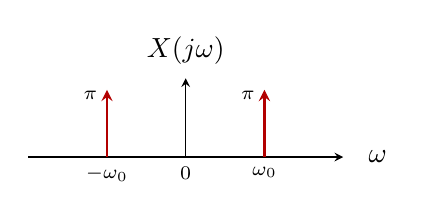
\begin{tikzpicture}
\begin{scope}	
    \begin{axis}[
		y=0.25cm,
		x=1cm,
		 clip=false,
		 xmin=-2,xmax=2,
		 xlabel= $\omega$,
		 ylabel={$X(j\omega)$},
		 ymin=0,ymax=4,
		 axis lines=middle,
		ticks=none,
		 every axis x label/.style={at={(ticklabel* cs:1.05)}, anchor=west,},
		every axis y label/.style={at={(ticklabel* cs:1.05)}, anchor=south,},
     ]		
		\addplot [mark=*, thick, mark size=1, y filter/.expression={y!=0 ? nan : y}] table[x=w,y=xw] {
w  xw
-1      3.414
1       3.414
};		
		\addplot+[red!70!black, thick, mark=none, y filter/.expression={y==0 ? nan : y}, quiver={u=0,v=-\thisrow{xw}}, stealth-] table[x=w,y=xw] {
w  xw
-1      3.414
1       3.414
};
		\node at (axis cs:1, pi) [anchor=east] {\scriptsize $\pi$ };	
		\node at (axis cs:-1, pi) [anchor=east] {\scriptsize $\pi$ };			
		\node at (axis cs:-1, 0) [anchor=north] {\scriptsize $-\omega_0$ };		
		\node at (axis cs:1, 0) [anchor=north] {\scriptsize $\omega_0$ };	
		\node at (axis cs:0, 0) [anchor=north] {\scriptsize $0$ };
    \end{axis}
\end{scope}

\end{tikzpicture} 